\documentclass{article}
\usepackage{graphicx} % Required for inserting images
\usepackage{graphicx} % Required for inserting images
\usepackage[left=0.5in, right=0.5in, top=0.5in, bottom=0.5in]{geometry}
\usepackage{amsmath}
\usepackage{amssymb}
\usepackage{amsfonts}
\usepackage{amsthm}
\usepackage{ulem}

% \title{Fractions, Decimals and Percentage}
\date{}

\begin{document}
\fontsize{13}{15} \selectfont %This is 13pt text with 15pt line spacing.

\text{Fractions, Decimals and Percentage.} \qquad Name: \hspace{5cm}  Class: \hspace{5cm}  \\
\vspace{10pt} 
\textit{(You must show your working.)  }
\vspace{5pt}

\hline
\vspace{10pt}
\text{(1)} \quad  Use equivalent fractions to solve: $ \displaystyle \frac{1}{6} + \displaystyle \frac{2}{3} $ \\
\vspace{10pt}

\hline
\vspace{10pt}
\text{(2)} \quad Multiply the numerator by the numerator and the denominator by the denominator. 
Then simplify (where needed).
$ \displaystyle \frac{1}{4} \times \displaystyle \frac{3}{5} $ \\
\vspace{10pt}

%\hline
%\vspace{10pt}
%\text{(3)} \quad $ \displaystyle \frac{2}{7} \div 3 $ \\
%\vspace{90pt}

\hline
\vspace{10pt}
\\[10pt] % Adds 10pt of vertical space
\text{(3)} \quad Multiply by the reciprocal of 3. \\ 
\vspace{20pt}
\( \displaystyle \frac{2}{7} \div \text{\Large 3} \) \\
\\[10pt] % Adds 90pt of vertical space

%begin{tabular}{l}
%\hline
%\\[10pt] % Adds 10pt of vertical space
%\text{(3)} \quad \( \displaystyle \frac{2}{7} \div \text{\Huge 3} \) \\
%\\[90pt] % Adds 90pt of vertical space
%\end{tabular}


\hline
\vspace{10pt}
\text{(4)} \quad Use the LCM method to solve: $ \displaystyle\frac{4}{5} + \displaystyle \frac{3}{7} $ \\
\vspace{10pt}
% \newpage

% \hline
\vspace{10pt}
\text{(5) \quad Work out } $ \displaystyle \frac{5}{6} \text{ of } \large 72 $  
\vspace{10pt}

%\hline
\vspace{10pt}
\text{(6) \quad Order the fractions from the smallest to the largest. } $ %\displaystyle \frac{5}{8} $ \\
\vspace{10pt}
\begin{center}
\text{(a)} $ \displaystyle \frac{1}{2} $  \qquad \text{ (b) } $ \displaystyle \frac{1}{4} $ \qquad  \text{ (c) } $ \displaystyle \frac{3}{4} $ \qquad  \text{ (d) } $ \displaystyle \frac{11}{16} $ 
\end{center}
\vspace{10pt}

%\hline
\vspace{10pt}

$
&\text{(7)} \quad \text{Make the fractions equivalent by multipying both the numerator and }  \\
\text{ denominator with the same number. } 
\displaystyle\frac{3}{5} = 
\genfrac{}{}{1pt}{0}{\fbox{\makebox[1em]{\rule{0pt}{1em}}}}{10} $
\vspace{10pt}

%\hline
%\vspace{10pt}
%&\text{(ii)} \quad 
%\genfrac{}{}{1pt}{0}{3}{\fbox{\makebox[1em]{\rule{0pt}{1em}}}} = \genfrac{}{}{1pt}{0}{\fbox{\makebox[1em]{\rule{0pt}{1em}}}}{12} = \genfrac{}{}{1pt}{0}{15}{\fbox{\makebox[1em]{\rule{0pt}{1em}}}} 


%\hline
%\\[10pt] % Adds 10pt of vertical space
%\text{(3)} \quad \( \displaystyle \frac{2}{7} %\div \text{\Large 3} \) \\
%\\[90pt] % Adds 90pt of vertical space

\item \quad Sort these numbers into the Venn diagram below. Remember, numbers that fit in both circles to be put at the point of intersection (the central oval). Numbers that do not belong to any circle should be put in the sample space (between the rectangle and the circles). 
\[ \frac{1}{2}, \hspace{1cm} \frac{6}{14}, \hspace{1cm} \Large4\frac{3}{5}, \hspace{1cm}  \frac{18}{5} \]
 \begin{center}
 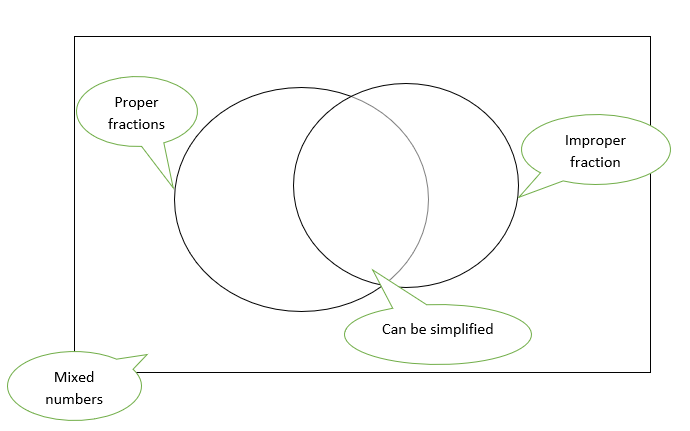
\includegraphics[width=12.5cm]{Frac_Dec_Per/VennC.png}
\end{center} 






\end{document}